\documentclass{article}
\usepackage{../preamble}
\usepackage{csquotes}

\title{Unit 12: The Gas Giants}
\author{Astronomy\footnote{Access for free at \href{\openstax}{\openstax}} \hspace{0.1ex} at Cypress Springs High School}
\date{Updated on \today}

\numberwithin{equation}{section}
\setcounter{section}{12}
\numberwithin{figure}{section}

\usepackage{fancyhdr}
\pagestyle{fancy}
\renewcommand{\headrulewidth}{0pt}
\renewcommand{\headruleskip}{0mm}
\fancyfoot[C]{Access for free at \href{\openstax}{\openstax} \hfill \thepage}
\fancyhead{}

\makenoidxglossaries

\begin{document}

\maketitle

\def\aMer{0.387}
\def\aVen{0.723}
\def\aEar{1}
\def\aMar{1.52}
\def\aJup{5.20}
\def\aSat{9.57}
\def\aUra{19.17}
\def\aNep{30.18}
\def\aAB{2.7}


\begin{center}
    \begin{tikzpicture}
        \begin{axis}[
            width=\textwidth,
            clip=true,
            axis equal image=true,
            xmin=-0.15,xmax=31,
            ymin=-\aJup,ymax=\aJup,
            axis line style={draw=none},
            ticks=none,
            cycle list={
                only marks,mark=*,fill=lightgray,draw=lightgray,mark size=0.1pt\\
                only marks,mark=*,fill=lightgray,draw=lightgray,mark size=0.1pt\\
              },
            domain=360-90:360+90,
            samples=1000,
        ]
            \draw[thick,black,fill=yellow] (0,0) %node[above right=2.5mm] {Sun} 
            circle (0.1);
            \draw (0,0) circle (\aMer);
            \draw[fill=black] (\aMer,0) circle (1pt); %node[right=1pt] {$\Mercury$};
            \draw (0,0) circle (\aVen);
            \draw[fill=black] (\aVen,0) circle (1pt); %node[right] {$\Venus$};
            \draw (0,0) circle (\aEar);
            \draw[fill=black] (\aEar,0) circle (1pt); %node[right] {$\Earth$};
            \draw (0,0) circle (\aMar);
            \draw[fill=black] (\aMar,0) circle (1pt); %node[right] {$\Mars$};
            \draw (0,0) circle (\aJup);
            \draw[fill=black] (\aJup,0) circle (2pt) node[right=1pt] {$\Jupiter$};
            \draw (0,0) circle (\aSat);
            \draw[fill=black] (\aSat,0) circle (2pt) node[right=1pt] {$\Saturn$};
            \draw (0,0) circle (\aUra);
            \draw[fill=black] (\aUra,0) circle (2pt) node[right=1pt] {$\Uranus$};
            \draw (0,0) circle (\aNep);
            \draw[fill=black] (\aNep,0) circle (2pt) node[right=1pt] {$\Neptune$};
            \addplot ({(\aAB+0.8*rand)*cos(x)},{(\aAB+0.8*rand)*sin(x)});
            %\node[right] at (3.5,0) {Asteroid Belt};
        \end{axis}
    \end{tikzpicture}
\end{center}

\subsection{Introduction}

The gas giants are the outer 4 planets in the solary system: Jupiter, Saturn, Uranus, and Neptune.

Some basic properties of the gas giants are summarized below:

\begin{center}
\begin{tabular}{|c|m{1.6cm}|m{1.6cm}|m{1.6cm}|m{2cm}|m{1.6cm}|m{1.6cm}|}
\hline
\textbf{Planet}	& \textbf{Distance (AU)} & \textbf{Period (years)} & \textbf{Diameter (km)} & \textbf{Mass (Earth = 1)} & \textbf{Density (\SI{}{g/cm^3})} & \textbf{Rotation (hours)}\\
\hline
Jupiter	& 5.2	& 11.9	& 142,800	& 318	& 1.3	& 9.9\\
Saturn	& 9.5	& 29.5	& 120,540	& 95	& 0.7	& 10.7\\
Uranus	& 19.2	& 84.1	& 51,200	& 14	& 1.3	& 17.2\\
Neptune	& 30.0	& 164.8	& 49,500	& 17	& 1.6	& 16.1\\
\hline
\end{tabular}
\end{center}

\subsection{Jupiter ($\Jupiter$)} \label{wX3zAX}

\begin{center}
    \begin{tikzpicture}[scale=1, transform shape]
        \clip (0.0,0.07) circle (1.76cm);
        \node at (-0.02,0.08) 
            {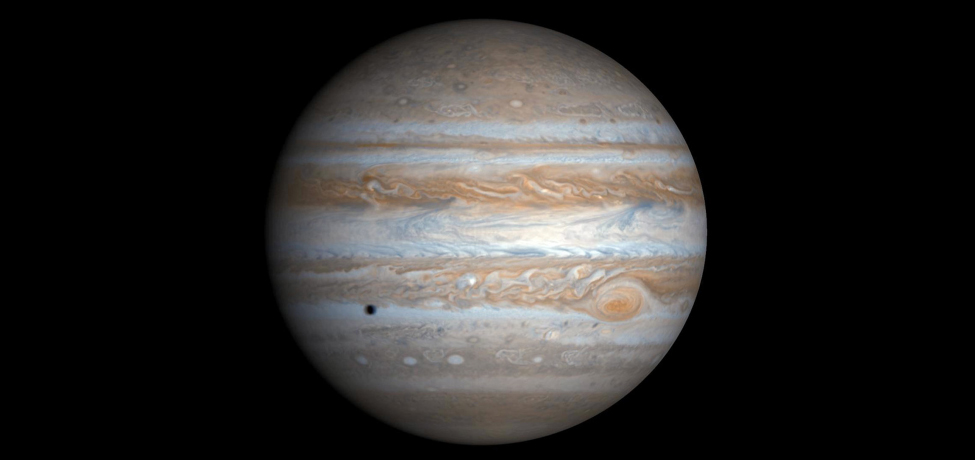
\includegraphics[width=8cm,trim={0cm 0mm 0cm 0mm}, clip]{Figures/Figure11.2.jpeg}};
            
    \end{tikzpicture}
    \captionsetup{type=figure,margin=1in,font=scriptsize}
    \captionof{figure}{The Cassini spacecraft imaged Jupiter on its way to Saturn in 2012. The giant storm system called the Great Red Spot is visible to the lower right. The dark spot to the lower left is the shadow of Jupiter’s moon Europa. (credit: modification of work by NASA/JPL)}
\end{center}

\clearpage

Robert Burnham, in \textit{The Reader's Digest Children's Atlas of the Universe}, writes

\begin{displayquote}
    The most massive of all the planets, Jupiter is an enormous ball of gas---mostly hydrogen and helium, like the Sun, along with small amounts of water, methane, and ammonia. This giant planet lacks a solid surface. The upper layers are gaseous but deeper down, as pressures and temperatures increase, the hydrogen and helium become more like a liquid. Deeper still, pressure makes the hydrogen behave like a liquid metal. At the center is a small, rocky core more than three times hotter than the surface of the Sun.

    A day on Jupiter lasts less than 10 hours. This rapid spin creates winds that blow at up to 300 miles per hour (\SI{500}{km/h}) and whip its colorful clouds into long bands. The light bands are called zones. The dark bands, known as belts, show deeper layers. Among the zones and belts are a number of oval spots. These are giant storms that thrive on the energy of the winds and heat from Jupiter's core. They can persist for years or even centuries---the biggest storm, the Great Red Spot, has been visible for at least 300 years. 

    In 1610, astronomer Galileo Galilei discovered Jupiter's four largest moons---Io, Europa, Ganymede, and Callisto. Today, we know of 16 moons, ranging from Ganymede, at 3,273 miles (\SI{5268}{km}) across, to Leda, at 10 miles (\SI{16}{km}) across.  In 1979, the Voyager 1 probe discovered that Jupiter also has a thin system of rings. These are mostly made of microscopic dust particles. 
\end{displayquote}



\subsection*{\ref{wX3zAX} Exercises}

\begin{exercise}
    What is the distance from the Sun to Jupiter, in astronomical units?
\end{exercise}

\begin{exercise}
    Jupiter rotates once on its axis every \rule{1cm}{0.15mm} hours.
\end{exercise}

\begin{exercise}
    How many years does it take Jupiter to orbit the Sun?
\end{exercise}

\begin{exercise}
    Jupiter is \rule{1cm}{0.15mm} times more massive than Earth.
\end{exercise}

\begin{exercise}
    True or False? Jupiter is the 5th most massive planet in the solar system.
\end{exercise}

\begin{exercise}
    What chemical elements is Jupiter mostly made of?
\end{exercise}

\begin{exercise}
    Recall that the terrestrial planets, like Mercury or Earth, have metallic cores. What kind of core does Jupiter have?
\end{exercise}

\begin{exercise}
    The dark bands on Jupiter are called \rule{2cm}{0.15mm}. The light bands are \rule{2cm}{0.15mm}.
\end{exercise}

\begin{exercise}
    What are the oval spots on Jupiter?
\end{exercise}

\begin{exercise}
    List some details about Jupiter's Great Red Spot.
\end{exercise}

\begin{exercise}
    Calculate how many years ago Galileo discovered the 4 largest moons of Jupiter.
\end{exercise}

\begin{exercise}
    \textit{Optional}: Calculate how many Jupiter-days are in one Jupiter-year.
\end{exercise}


\clearpage
\subsection{Saturn ($\Saturn$)} \label{qBDig}

\begin{center}
    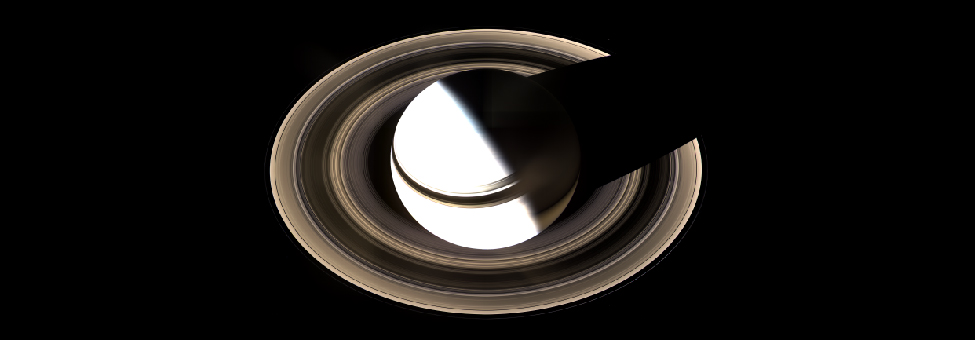
\includegraphics[width=6cm,trim={3cm 0cm 3cm 0cm},clip]{Figures/Figure7.7.jpeg}
    \captionsetup{type=figure,margin=1in,font=scriptsize}
    \captionof{figure}{\textbf{Saturn and Its Rings.} This 2007 Cassini image shows Saturn and its complex system of rings, taken from a distance of about 1.2 million kilometers. This natural-color image is a composite of 36 images taken over the course of 2.5 hours. (credit: modification of work by NASA/JPL/Space Science Institute)}
\end{center}

In \textit{Reader's Digest Children's Atlas of the Universe}, writing in 2000, Robert Burnham explains:

\begin{displayquote}
    Saturn is known as the Ringed Planet. Jupiter, Uranus, and Neptune also have rings, but Saturn's are the most magnificent. From Earth, we can see what look like three broad, smooth rings. The A ring is the outside one. Next comes the Cassini division, a dark gap 2,900 miles (\SI{4670}{km}) wide. The B ring is the widest and brightest, 16,000 miles (\SI{25750}{km}) across. The narrower C ring, just inward, appears pale and semi-transparent. 

    \vspace{1em}

    Three spacecraft---Pioneer 11 and Voyagers 1 and 2---have visited Saturn since 1979. They revealed that the rings are made up of thousands of ringlets, each made up of icy chunks. Even the empty-looking Cassini division contains many particles. Scientists think that the rings are the remains of several smashed moons. As time passes, ring particles collide and slowly spiral into Saturn. Millions of years from now, the rings will be gone.

    \vspace{1em}

    Saturn seems like a pale, cool copy of Jupiter. It has no solid surface and, like Jupiter, is nearly all hydrogen and helium, with traces of other gases such as methane and ammonia. Although Saturn is nearly as big as Jupiter, it has only 30 percent as much mass. A bit like a giant marshmallow, Saturn would float if you could find a large enough ocean. 

    \vspace{1em}

    The winds at Saturn's equator blow at more than 1,000 miles per hour (\SI{1600}{km/h})---much faster than Jupiter's winds. Saturn has fewer storms than Jupiter does because it has less internal heat, but large white clouds of ammonia ice crystals break out at its equator about every 30 years. 

    \vspace{1em}

    Outside the main rings orbit 18 moons, ranging from Titan, 3,200 miles (\SI{5150}{km}) in diameter, to Pan, just 12 miles (\SI{20}{km}) across. Titan is the target for the Huygens probe carried by the Cassini spacecraft, due to reach Saturn in 2004.
\end{displayquote}

\subsection*{\ref{qBDig} Exercises} 

\begin{exercise}
    In what way is Saturn like a giant marshmallow?
\end{exercise}

\begin{exercise}
    List the spacecraft that have visited Saturn.
\end{exercise}

\begin{exercise}
    What is the Cassini division? Draw a sketch to explain.
\end{exercise}

\begin{exercise}
    What is the probable origin of Saturn's rings?
\end{exercise}

\begin{exercise}
    Will its rings be there forever? Explain.
\end{exercise}

\begin{exercise}
    Between Saturn and Jupiter, which has more storms? Which has faster winds?
\end{exercise}

\begin{exercise}
    Identify Saturn's largest moon.
\end{exercise}

\begin{exercise}
    What is this gas giant mostly made of? List the top 2 elements.
\end{exercise}

\clearpage

\subsection{Uranus ($\Uranus$)} \label{ejwEWF}

\begin{center}
    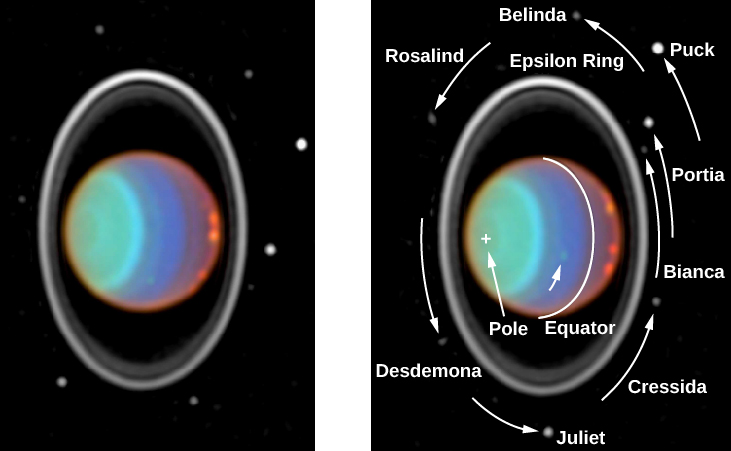
\includegraphics[width=5.5cm]{Figures/Figure11.5.jpeg}
\end{center}

Robert Burnham, in \textit{Reader's Digest Children's Atlas of the Universe}, writes:

\begin{displayquote}
    In 1781, William Herschel looked through his telescope and found Uranus, the first planet discovered in modern times. Uranus has a diameter about four times greater than Earth's, but it orbits so far from the Sun that Herschel and other observers could tell little about the planet. Most of what we now know about Uranus was learned from the Voyager 2 spacecraft flyby in 1986. 

    \vspace{1em}

    Uranus might be called the planet-on-its-side---Earth's axis tilts 23.5 degrees to its orbit, but Uranus's axis tips almost 98 degrees. When Voyager 2 flew past, Uranus's south pole was pointing almost directly at the Sun, and the northern hemisphere was in darkness. Voyager saw a bland, blue-green Uranus without any features. Scientists using the Hubble Space Telescope are now seeing signs of storms in Uranus's northern hemisphere as it emerges from its long, dark winter.

    \vspace{1em}

    The blue-green color of Uranus comes from traces of methane it its upper atmosphere. The methane reflects the blue wavelengths of sunlight and absorbs the red. Most of Uranus, however, is hydrogen and helium, like the Sun. And like the other gas-giant planets, it has no solid surface.

    \vspace{1em}

    In 1977, astronomers watched a star wink on and off before disappearing behind Uranus. This revealed that Uranus has a set of narrow, dark rings. Eleven rings are now known. The dark gray ring particles are a few inches to 10 yards (10 cm to 10 m) across. 

    \vspace{1em}

    Uranus has five large moons, including Miranda, which has a surface unlike any other moon in the solar system. In recent years, many smaller moons have been discovered. There are at least 15 of these dark asteroid-like objects. 
\end{displayquote}


\subsection*{\ref{ejwEWF} Exercises}

\begin{exercise}
    Uranus was unknown to the ancients and at some point had to be discovered via telescope. Who discovered Uranus and in what year was the discovery made?
\end{exercise}

\begin{exercise}
    If someone was born on the year that Voyager 2 visited Uranus, how old would they be now?
\end{exercise}

\begin{exercise}
    Identify the curious and unique property of the tilt of the axis of Uranus.
\end{exercise}

\begin{exercise}
    In 1986, which hemisphere of the planet was going through a long and dark winter? How did scientists conclude that it must have been winter there?
\end{exercise}

\begin{exercise}
    Identify the gas in the atmosphere that gives Uranus its blue-greenish color.
\end{exercise}

\begin{exercise}
    True or False? Uranus is only gas giant that has a solid surface.
\end{exercise}

\begin{exercise}
    What was the mysterious ``star'' winking behind the planet?
\end{exercise}

\begin{exercise}
    How many rings does this planet have?
\end{exercise}

\begin{exercise}
    Name one of Uranus's moons.
\end{exercise}

\begin{exercise}
    Calculate how long it's been since the discovery of Uranus.
\end{exercise}

\clearpage

\subsection{Neptune ($\Neptune$)} \label{yka1VU}

\begin{center}
    \begin{tikzpicture}[scale=1, transform shape]
        \clip (0.0,-0.05) circle (1.76cm);
        \node at (0,0.0) 
            {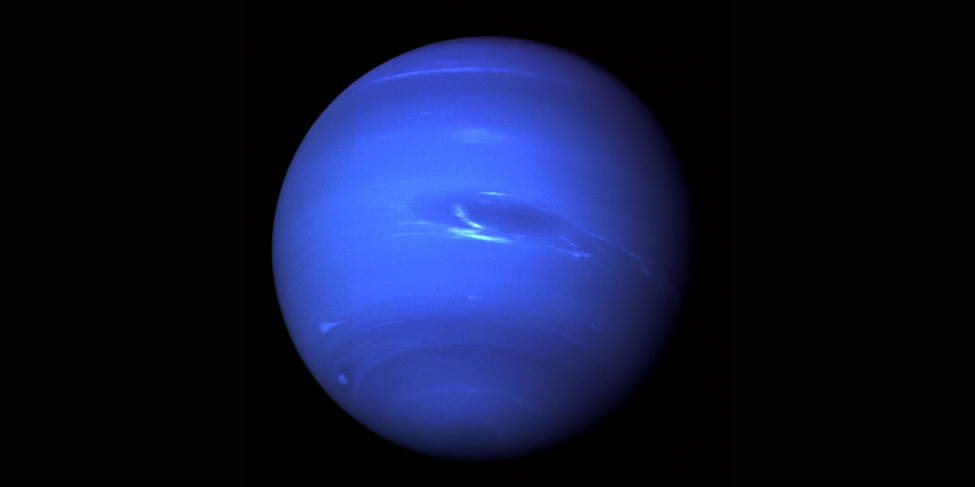
\includegraphics[width=8cm,trim={0cm 0mm 0cm 0mm}, clip]{Figures/Figure11.15.jpeg}};
        
    \end{tikzpicture}
    \captionsetup{type=figure,margin=1in,font=scriptsize}
    \captionof{figure}{The planet Neptune is seen here as photographed by Voyager in 1989. The blue color, exaggerated with computer processing, is caused by the scattering of sunlight in the planet's upper atmosphere. (credit: modification of work by NASA)
}
\end{center}

In \textit{Reader's Digest Children's Atlas of the Universe}, Robert Burnham writes:

\begin{displayquote}
    Neptune is the Sun's last gas-giant planet. It was first spotted in 1846 after astronomers noticed that Uranus wasn't moving along its orbit exactly as it should. Guessing that an unknown planet was orbitting farther out and influencing Uranus, the astronomers John Couch Adams in England and Urbain Leverrier in France independently calculated where the new planet might be. When observers Johann Galle and Heinrich d'Arrest checked, they found the new planet right where Adams and Leverrier had predicted.

    \vspace{1em}

    Since Neptune orbits far from Earth, little was known about it until the Voyager 2 spacecraft paid a flyby visit in 1989. The spacecraft showed that Neptune is a cold, blue echo of Uranus, with some important differences. Like Uranus, Neptune is a ball of hydrogen, helium, and methane. The tilt of Neptune's axis (29.6 degrees) is not as extreme as Uranus's, so its seasonal changes are less dramatic. Neptune has raging storms and clouds. Voyager photographed a giant storm known as the Great Dark Spot and a fast-moving cloud of methane ice crystals called the Scooter. Observations from Earth show that storms come and go over the years, probably driven by Neptune's internal heat. 

    \vspace{1em}

    Two Neptunian moons were known before Voyager. Its flyby added six. They range from Triton, with a diameter of 1,681 miles (\SI{2706}{km}), to Naiad, just 36 miles (\SI{58}{km}) wide. Triton has erupting geysers, but the other moons are inactive worlds.

    \vspace{1em}

    Astronomers discovered the rings of Neptune in 1984. They found that one of the six rings has clumps in it, caused perhaps by moons that are yet to be discovered.
\end{displayquote}

\subsection*{\ref{yka1VU} Exercises}

\begin{exercise}
    In what year did Voyager 2 visit Neptune?
\end{exercise}

\begin{exercise}
    Calculate how many years have passed since the discovery of Neptune.
\end{exercise}

\begin{exercise}
    Neptune's orbital period is 165 years---that's how long it takes to orbit the Sun. How many trips around the Sun has Neptune completed since the year of its discovery?
\end{exercise}

\begin{exercise}
    To which of the 8 planets in the solar system is Neptune most similar?
\end{exercise}

\begin{exercise}
    Explain the Scooter.
\end{exercise}

\begin{exercise}
    What is the name of the giant storm on Neptune?
\end{exercise}

\begin{exercise}
    Draw a sketch of what you think the geysers on Triton could look like. (If you're not sure what a \textit{geyser} is, look it up.)
\end{exercise}

\begin{exercise}
    True or False? Neptune has rings.
\end{exercise}




\end{document}